\section{Aufgabenstellung}
In diesem Versuch sollen grundlegende Kentnisse der elektronischen Datenverarbeitung mittels FPGA, sowie die Konfiguration dieser mittels VHDL vermittelt werden.
Dazu sollen folgende Module programmiert, simuliert und zum Teil auf ein vorliegendes FPGA übertragen werden:
\begin{itemize}
\item mehrere einfache Logikschaltungen (Details sind in der Auswertung zu finden)
\item Ein Modul \glqq LoHi Detect\grqq{}
\item Ein Modul \glqq Max Find\grqq{} welches das Maximum des Inputs ausgibt
\item Ein Modul \glqq Filter\grqq{} das einen Wiener Filter zur Unterdrückung des Rauschens im Input implementiert
\item Eine Uhr die \SI{9}{\s} auf einer Digitalanzeige zählt und sich danach zurücksetzt
\item Ein Modul \glqq ssd\grqq{} das einen vierstelligen Input auf einem digitalenm Display anzeigt
\end{itemize}
Die vier Module sollten im Anschluss in einem Modul \glqq top\grqq{} zusammengeschlossen werden, welches als Filter für einen elektronischen Impuls, wie er bei einem Kalorimeter auftritt, fungieren soll.

\section{Theorie}

\subsection{FPGA}
Bei Field Programmable Gate Arrays (FPGA) handelt es sich um spezielle Integrierte Schaltkreise (IC), die nach Herstellung vom Benutzer frei konfiguriert werden können.
Dies trennt sie von herkömmlichen Application Specific Integrated Circuits (ASIC) welche nach Herstellung nicht abgeändert werden können.

Vorteile von FPGA, die sie so interessant in der Anwendung machen, sind unter anderem ihre bereits erwähnte Konfigurierbarkeit, gute Parallelisierbarkeit, ein geringes Risiko von Fehldesigns, die schnelle Implementierung neuer Designs und recht niedrige Kosten für geringe Stückzahlen.
Gleichzeitig existieren aber auch diverse Nachteile, wie geringere Taktfrequenzen als ASICS, geringere Logikdichten, höherer Stromverbrauch sowie eine allgemein geringere Strahlenhärte.

FPGA besitzen Eingangs- und Ausgangssignale (I/O-Port).
Die Eingangssignale können mithilfe von Logikblöcken verbunden werden und so ein gewünschtes Ausgangssignal, abhängig vom Eingang, erzeugt werden.
Um die Rekonfigurierbarkeit von FPGA zu ermöglichen, werden \glqq Schalter\grqq{} zwischen den Logikblöcken eingefügt, die durch anlegen einer Spannung manipuliert werden können.
Ein Beispiel für die Schaltung zwischen Logikblöcken ist in Abb. \ref{schalter} zu sehen.
\begin{figure}[h]
  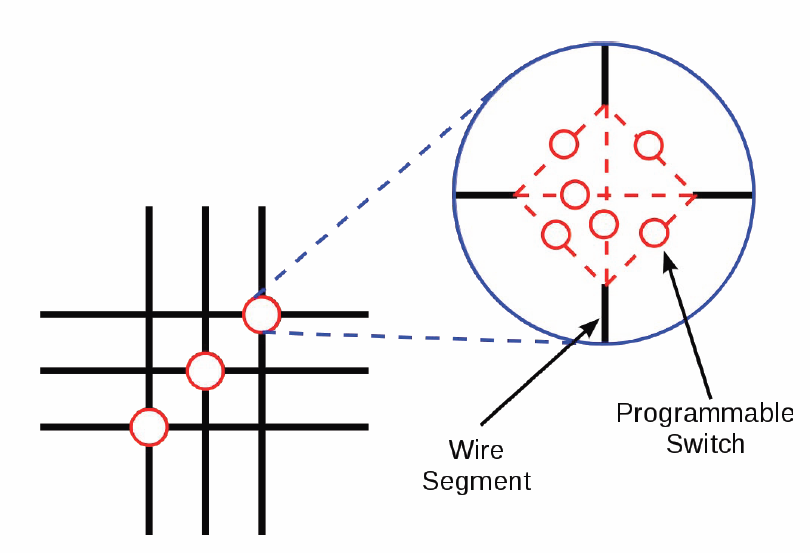
\includegraphics[width=\linewidth]{../Daten/schalter.png}
  \caption{rekonfigurierbare Schalter zwischen Logigblöcken}
  \label{schalter}
\end{figure}
Um ein FPGA auf gewünschte Art zu konfigurieren, müssen Hardware-Programmiersprachen (\glqq Hardware Description Language\grqq{} oder HDL) verwendet werden.
Bei FPGA stellen diese eine Art \glqq Schaltplan\grqq{} der logischen Verknüpfungen innerhalb des FPGA dar.
Hierbei ist zu beachten, dass bei der Konfiguration auch wirklich Signale vom Eingang zum Ausgang geleitet und dabei mittels logischer Funktionen manipuliert werden.
Aufgrunddessen ist auch die gute Parallisierbarkeit des FPGA leicht zu verstehen.
Umfang sowie Geschwindigkeit der Konfiguration ist hier jedoch prinzipiell durch Logikdichte sowie Signallaufzeit des FPGA beschränkt.

\subsection{Kalorimeter}
Kalorimeter dienen in der Teilchenphysik zur Messung der Energie einfallender Teilchen.
Die Idee hinter diesen ist es, die einfallenden Teilchen (z. B. Elektronen oder Photonen) vollständig im Kalorimeter zu stoppen und die dabei freigesetzte Energie zu messen.
In der Praxis geschieht dies, z. B. bei einem elektromagnetischen Kalorimeter, mit einem Verbund aus mehreren Absorber- und Ausleseschichten, an die eine Hochspannung geschlossen ist.
Innerhalb der Absorberschichten geben die Teilchen Energie ab, wobei das Absorbermaterial ionisiert wird.
Durch die Hochspannung werden die so freigesetzten Ladungen abgesaugt, wodurch ein elektrischer Impuls entsteht.
In der Theorie bewegen sich hochenergetische Teilchen nahezu mit Lichtgeschwindigkeit durch den Kalorimeter und ionisieren entlang ihres Weges, was zu Dreiecksimpulsen führt.
Das heißt die gemessene Spannung springt auf einen Wert, der abhängig von der Energie des Teilchens ist, und fällt dann linear ab.
In der Praxis gibt es im wesentlichen drei Störquellen, die den Impuls verzerren:
\begin{itemize}
\item Eine ist rein stochastischer Natur und verhält sich proportional zu $\frac{1}{\sqrt{E}}$.
Diese entsteht dadurch, dass die Genauigkeit eines Kalorimeters von der Bestimmung der Anzahl ionisierter Teilchen abhängig ist, welche wiederum einer Poisson-Statistik genügt.

\item Desweitern gibt es eine konstante Störquelle durch Inhomgenitäten im Detektor sowie Energieverluste der Teilchen außerhalb der Absorberschichten.

\item In diesen Versuch von besonderem Interesse ist das elektrische Rauschen, das sich unweigerlich im Detektor ergibt.
Dieses entsteht zum Beispiel durch Untergrundstrahlung oder das Pile-Up, das entsteht, wenn eine Überlagerung mehrerer zu detektierender Ereignisse im Detektor stattfindet (siehe zum Beispiel Abb. \ref{pileup}).
Der hierbei entstehende Fehler ist dabei proportional zu $\frac{1}{E}$, wobei E die im Kalorimeter deponierte Energie ist.
\end{itemize}

\begin{figure}[h]
  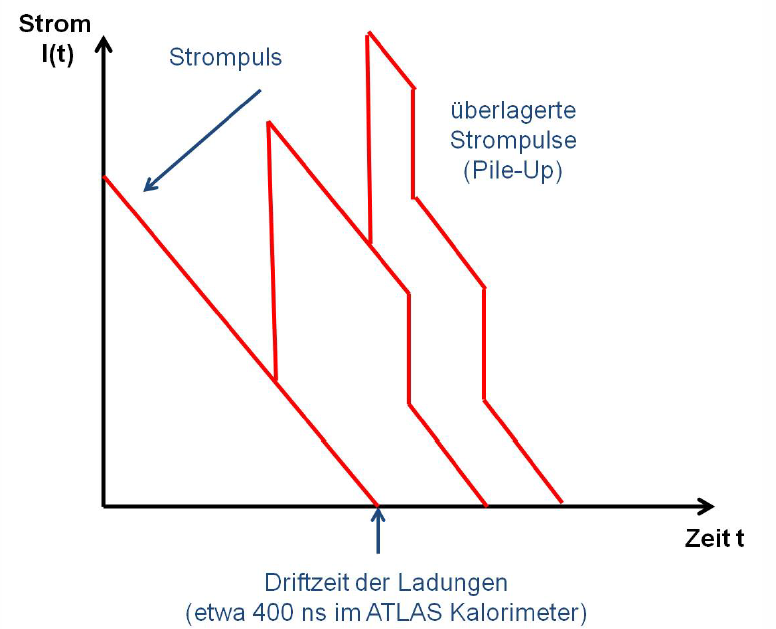
\includegraphics[width=\linewidth]{../Daten/pileup.png}
  \caption{Beispielhafte Darstellung eines Pile-Ups}
  \label{pileup}
\end{figure}
Für die Analyse der Detektoren ist es wesentlich dieses Rauschen zu unterdrücken.
Eine Möglichkeit dafür besteht in der Verwendung digitaler Filteralgorithmen, welche z. B. im FPGA implementiert werden können.
Um die Untergrundstrahlung bzw. das Pile-Up, welche zu einem ständigen Anwachsen des Impulses bzw. einem verschieben der Nulllinie führen, zu unterdrücken, wird der Impuls durch eine Kombination von RC- bzw. CR-Schaltungen (R = Widerstand, C = Kondensator) geführt.
Diese Schaltungen \glqq integrieren\grqq{} bzw. \glqq differenzieren\grqq{} den Impuls und wirken gleichzeitig als Frequenzfilter.

Als nächstes wird auf den Impuls eine \glqq digitale Filterung\grqq{} angewandt.
Dabei werden die nun diskreten Spannungswerte mit speziellen, vorher bestimmten Konstanten multipliziert, was das Rauschen im Impuls unterdrückt (ohne Beweis).
Aufsummieren der gefilterten Werte gibt nun Energiewerte (also die Pulshöhe), die als Ausgabe des FPGA dienen können.
Damit ergibt sich die Energie zu:
\begin{equation}
E = \sum_{i = 1}^{N} a_i S_i
\end{equation}
Hier sind $a_i$ die Filterkonstanten und $S_i$ die Impulsbeträge.

Da dieser Prozess in einem modernen Kalorimeter jede Sekunde für große Datenmengen gleichzeitig durchgeführt werden muss, sind FPGA wegen der bereits erwähnten Parallelisierbarkeit für diese Filter prädestiniert.
In diesem Versuch soll daher eine digitale Filterung, wie sie im vorherigen Absatz beschrieben wurde, konfiguriert werden.


\section{Versuchsaufbau}
In diesem Versuch wird ein Elvis II Entwicklungsboard der Firma National Instruments verwendet (siehe Abb. \ref{board}).
Dieses verfügt neben einem FPGA über einen An/Aus-Schalter, LEDs, vier ansteuerbare Siebensegmentanzeigen, mehrere Schalter sowie eine USB-Verbindung.

\begin{figure}[h]
  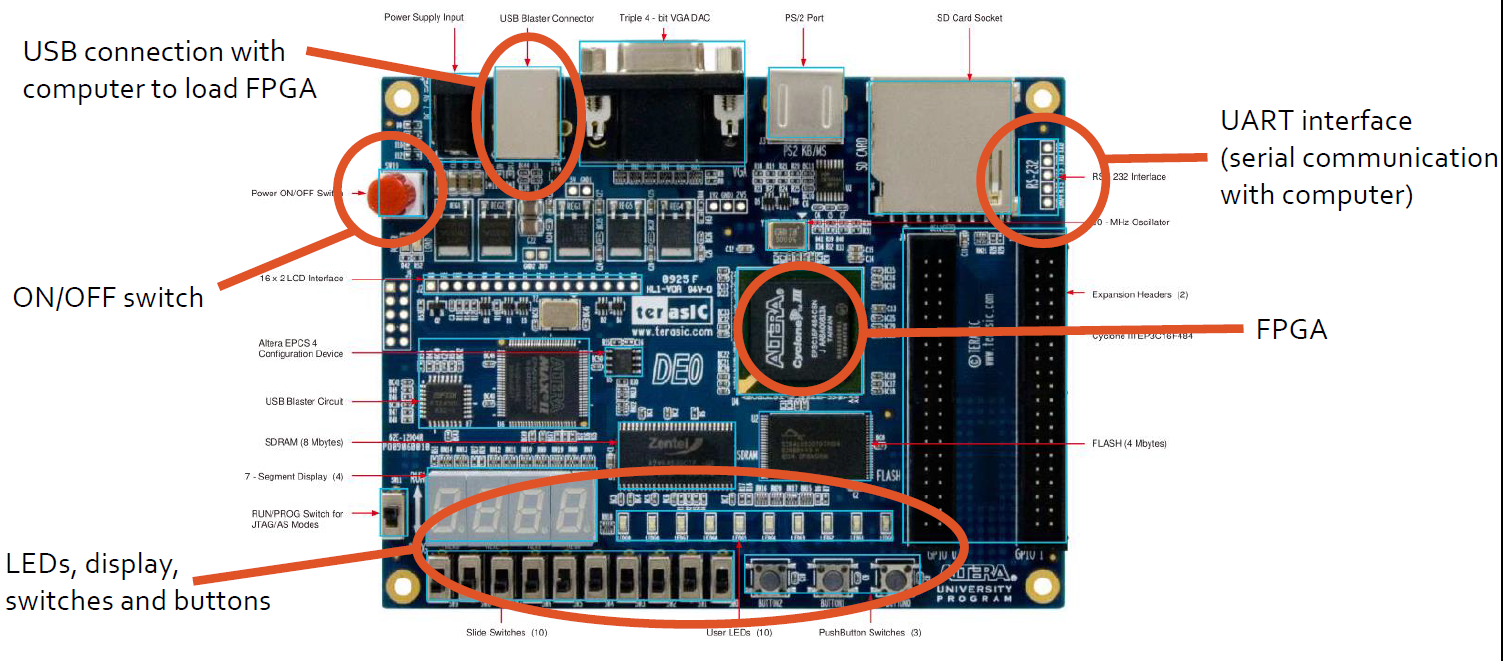
\includegraphics[width=\linewidth]{../Daten/board.png}
  \caption{Elvis II Entwicklungsboard}
  \label{board}
\end{figure}

Zur Konfiguration des FPGA werden Programmcodes in der Programmiersprache VHDL geschrieben (Details zu dieser sind in der Auswertung zu finden).
Diese Skripte werden danach auf einem PC simuliert, um Funktionalität zu gewährleisten und eventuelle Fehlerquellen zu finden.
Wenn keine vorhanden sind, wird das Skript auf das FPGA übertragen wobei dieses synthetisiert wird.
Einzelne Skripte konnten dann direkt auf dem FPGA getestet werden.
